%%%%%%%%%%%%%%%%%%%%%%%%%%%%%%%%%%%%%%%%%
%  Design Documentation for CSEE4840
%  Objetive: Explain what I did and how, so someone can continue with the investigation
%
% Important note:
% Chapter heading images should have a 2:1 width:height ratio,
% e.g. 920px width and 460px height.
%
%%%%%%%%%%%%%%%%%%%%%%%%%%%%%%%%%%%%%%%%%

%----------------------------------------------------------------------------------------
%	PACKAGES AND OTHER DOCUMENT CONFIGURATIONS
%----------------------------------------------------------------------------------------

\documentclass[twoside,12pt,fleqn]{book} % Default font size and left-justified equations

\usepackage[top=3cm,bottom=3cm,left=3.2cm,right=3.2cm,headsep=10pt,letterpaper]{geometry} % Page margins
\usepackage[document]{ragged2e}
\usepackage{xcolor} % Required for specifying colors by name
\definecolor{ocre}{RGB}{52,177,201} % Define the orange color used for highlighting throughout the book

% Font Settings
\usepackage{avant} % Use the Avantgarde font for headings
%\usepackage{times} % Use the Times font for headings
\usepackage{mathptmx} % Use the Adobe Times Roman as the default text font together with math symbols from the Sym­bol, Chancery and Com­puter Modern fonts

\usepackage{microtype} % Slightly tweak font spacing for aesthetics
\usepackage[utf8]{inputenc} % Required for including letters with accents
\usepackage[T1]{fontenc} % Use 8-bit encoding that has 256 glyphs
% Bibliography
\usepackage[style=alphabetic,sorting=nyt,sortcites=true,autopunct=true,babel=hyphen,hyperref=true,abbreviate=false,backref=true,backend=biber]{biblatex}
\usepackage{csquotes}
\addbibresource{bibliography.bib} % BibTeX bibliography file
\defbibheading{bibempty}{}

\input{structure} % Insert the commands.tex file which contains the majority of the structure behind the template


\begin{document}

%----------------------------------------------------------------------------------------
%	TITLE PAGE
%----------------------------------------------------------------------------------------

\begingroup
\thispagestyle{empty}
\AddToShipoutPicture*{\put(0,0){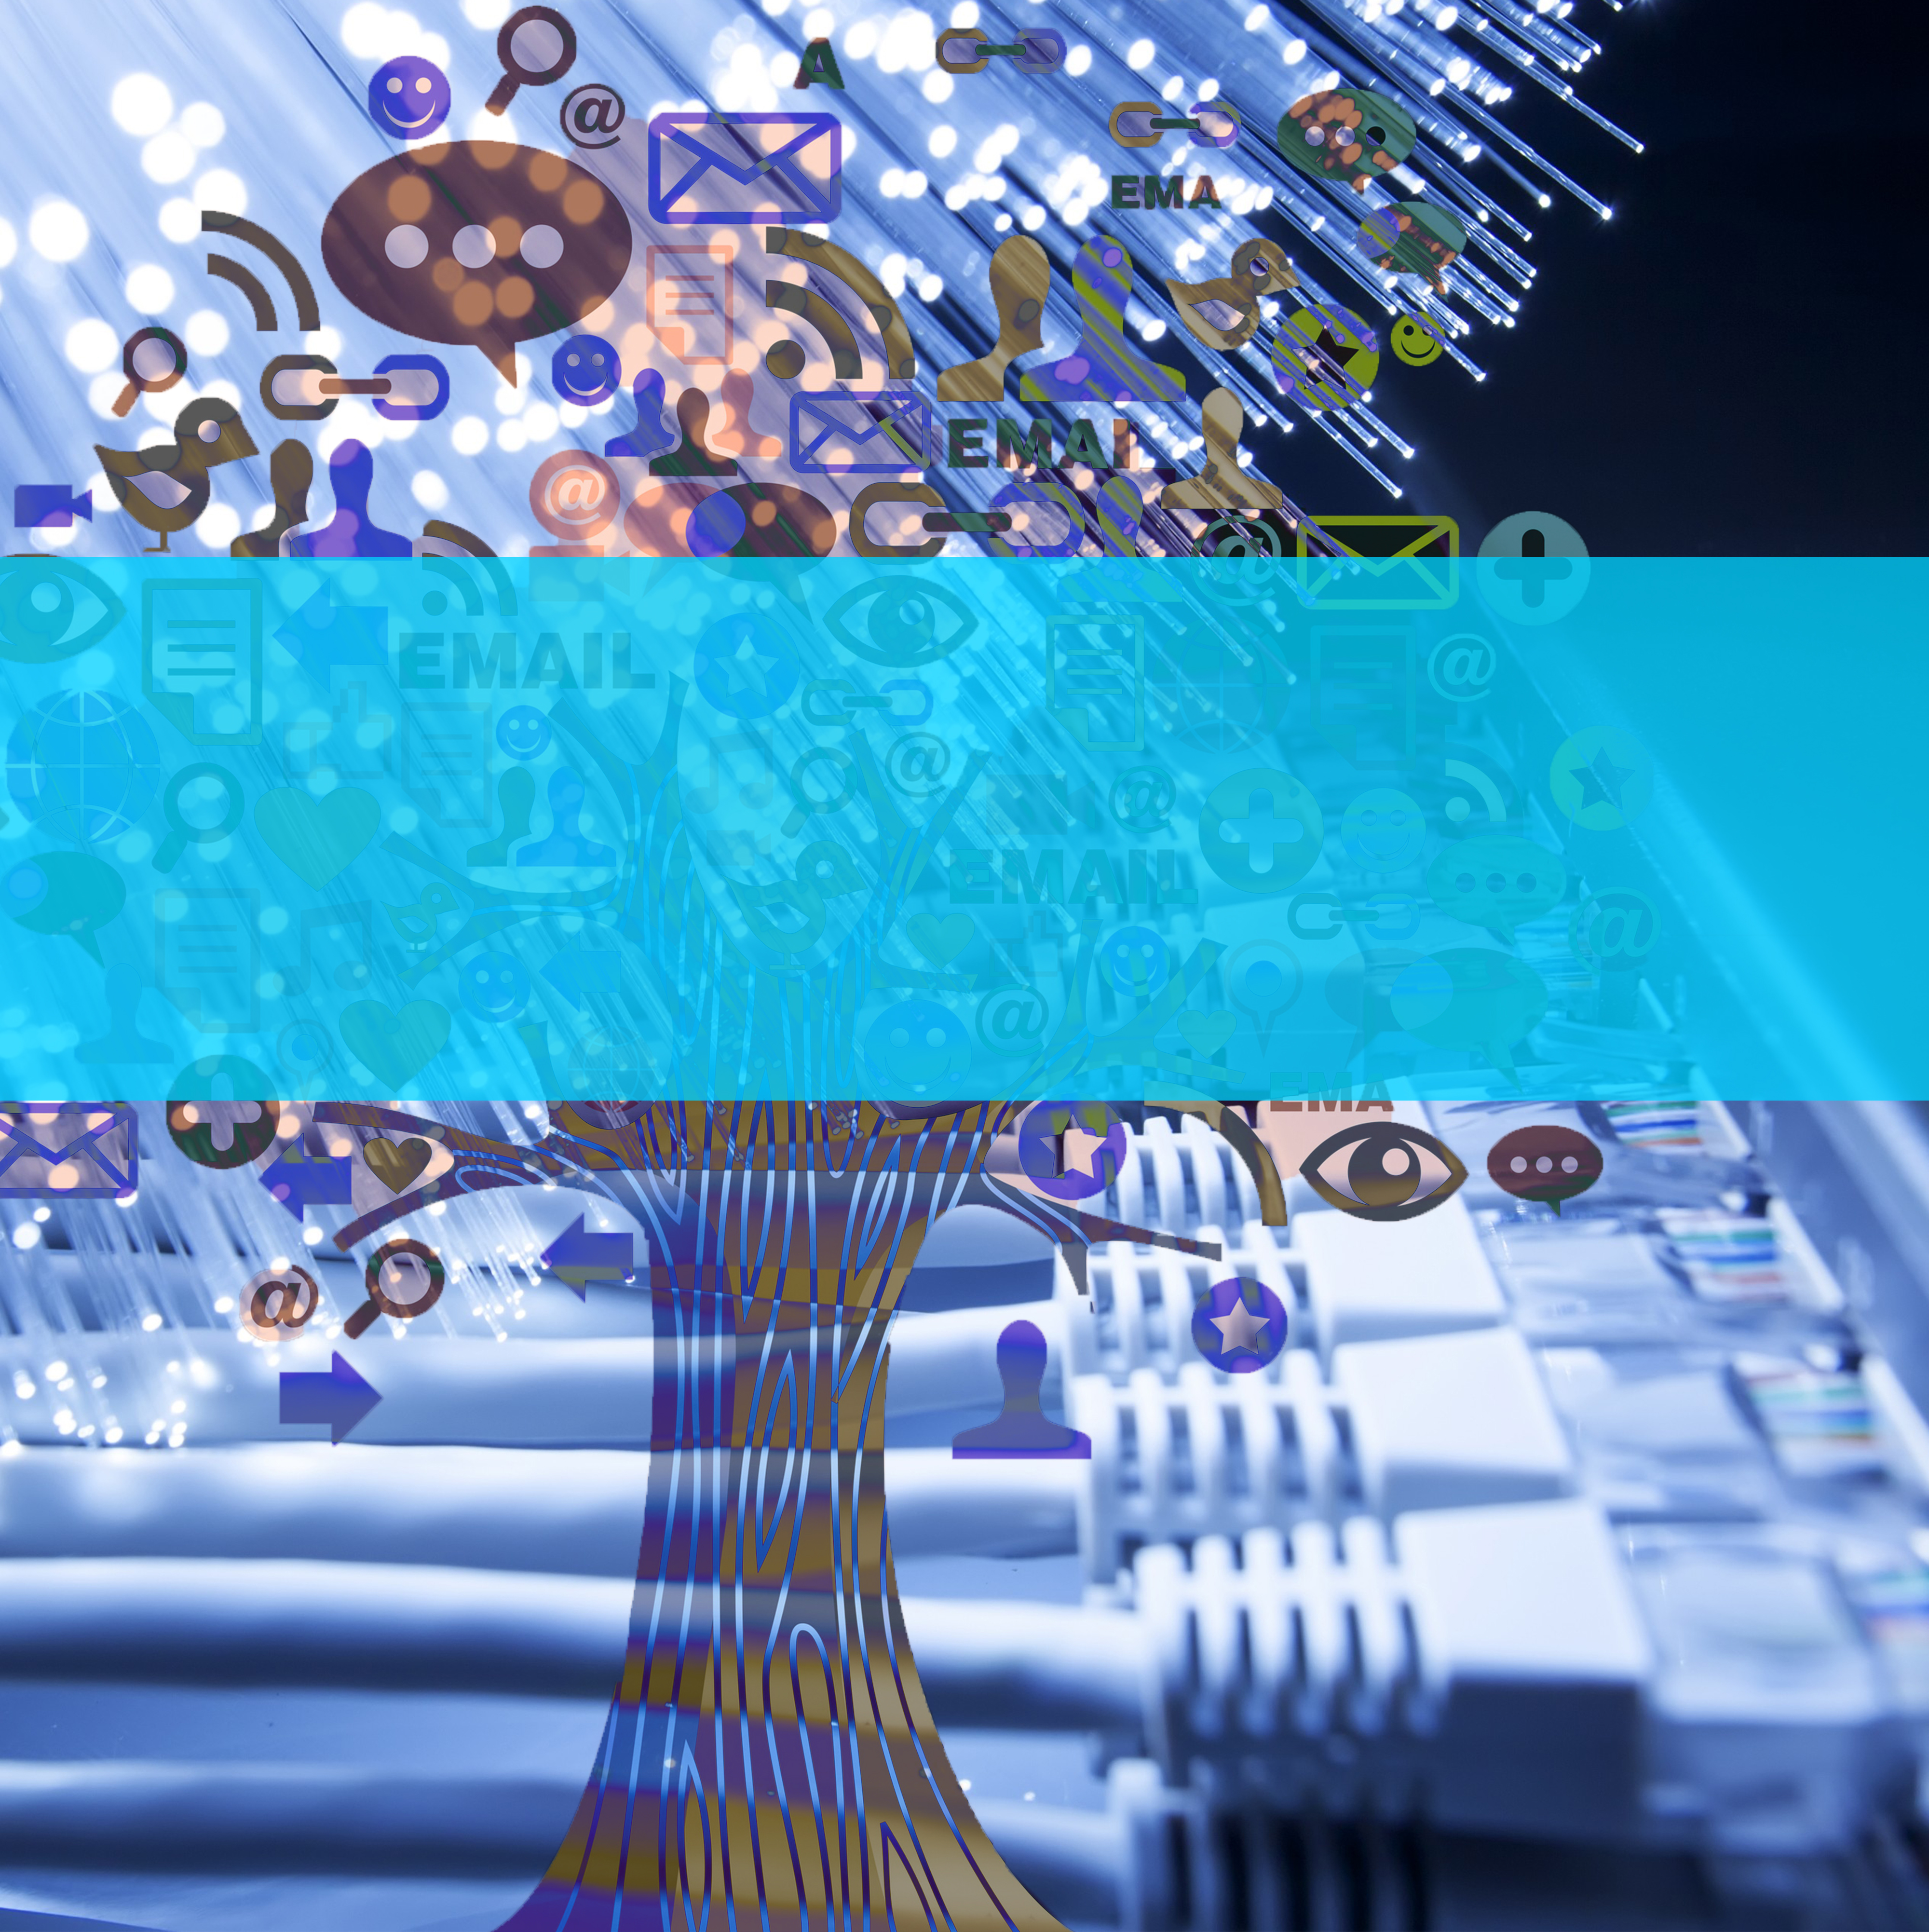
\includegraphics[height=\paperheight]{cover_page.jpg}}} %Image background
\centering
\vspace*{5cm}
\par\normalfont\fontsize{35}{35}\sffamily\selectfont
\textbf{Switch ON}\\
{\LARGE An FPGA based Switch}\par % Book title
\vspace*{1cm}
{\Huge Ayush Jain(aj2762)\\ Donovan Chan(dc3095)\\ Shivam Choudhary(sc3973)}\par % Author name
\endgroup

%----------------------------------------------------------------------------------------
%	TABLE OF CONTENTS
%----------------------------------------------------------------------------------------
\newpage
\let\cleardoublepage\clearpage
\chapterimage{contents.png} % Table of contents heading image

\pagestyle{empty} % No headers

\tableofcontents % Print the table of contents itself
%\cleardoublepage % Forces the first chapter to start on an odd page so it's on the right
\pagestyle{fancy} % Print headers again

%----------------------------------------------------------------------------------------
%	CHAPTER 1
%----------------------------------------------------------------------------------------

\chapterimage{intro.jpg} % Chapter heading image
%\let\cleardoublepage\clearpage
\chapter{Introduction}

\section{Aim} 
\index{Aim}
\justify
The idea is to create a FPGA based \texttt {switching fabric}. The main focus of the project is in optimising the throughput of a network switch through the implementation of a scheduler. Decoding of actual incoming packets will not be considered in this project.\footnote{When we say we won't be decoding actual incoming packets we mean that we don't care if the packet is actually a proper IP packet.} Therefore the packets being generated will contain randomly generated payload and a header that determines the output port.

\section{Overview}\index{Overview}
We will be creating a scheduling algorithm that optimizes the throughput\footnote{We define throughput to be the number of packets coming out from the output port in \texttt{one clock cycle.}}. We will be implementing the crossbar switch and the scheduler in the FPGA. Our packet generator software would interface with the FPGA memory and would be used as a simulator for generating random packets destined for different output ports. Furthermore to evaluate that the scheduler routed the packet properly, we would be designing a validator which would interface with the output memory of the FPGA and would determine if the packets were correctly routed.

\section{Evaluation of Idea}\index{Evaluation of Project}
We would do a comparative study between the throughput obtained by running a scheduling algorithm and one without it. Though we know that the scheduling algorithm will be faster but we would like to know by how much. Benchmark tests will be used to evaluate the validity of the scheduler and its effectiveness in maximising throughput of the network switch.

\let\cleardoublepage\clearpage
\chapterimage{hardware.jpeg}

\chapter{Hardware Design}

\section{Network Fabric}\index{Network Fabric}
A network switching fabric is the hardware topology of the network that is laid out and is responsible for routing the input packet to its respective output port. The network fabric being employed in this project will be the Crossbar architecture. The crossbar architecture is basically a network topology that is in the form of a matrix as shown in Figure \ref{fig:crossbar_illustration} below: 
    \begin{figure}[ht]
        \centering
        \includegraphics[width=0.65\textwidth]{Crossbar_Architecture.jpg}
        \caption{Illustration of the Crossbar Architecture that will be responsible for the network switching fabric}
        \label{fig:crossbar_illustration}
    \end{figure}

So there is 1-1 matching between the input port and the output port. The Input(1,2,3) denotes the line cards which will be receiving the packets destined to different output port but one which is not known beforehand.
\subsection{Crossbar Switch Model}
In this project, we will be using a single layer 4$\times$4 topology with 4 inputs and 4 outputs. The Figure \ref{fig:crossbar_illustration} above illustrates how every input is being connected to every output by the intersections of the matrix, termed crosspoints. The implementation of the crossbar switch model will be done on the FPGA. Each input to output connection is completely independent of each other and can therefore support simultaneous communications, except in the case when two ports wish to use the same output port.
\subsubsection{How the Crossbar Switch Works}
The crossbar switch architecture works in a similar way to that of active addressing in an LED(Light emitting diode) matrix. The inputs are connected to every output by lines that can be turned on and off depending on the destination of the source packet. For example in Figure \ref{fig:crossbar_illustration}, the orange line shows how the input 1 is able to send a packet through the network fabric to output 2 by turning on it's horizontal line and the vertical line that corresponds to output 2. As mentioned earlier, the lines are independent of one another and therefore in a single time slot, both input 1 and input 2 can send packets to outputs 2 and 3 respectively without colliding. Theoretically and in some cases practically it is possible to get \texttt{n}\footnote{where n is number of output ports,in this case 4} number of packets in the output.
\par\vspace{\baselineskip}
\begin{figure}[ht]
    \centering
    \includegraphics[width=0.60\textwidth]{HOL_Blocking.jpg}
    \caption{Illustration of the HOL blocking in effect}
    \label{fig:HOL_Blocking}
\end{figure}
It can therefore be seen that the primary concern with congestion in the network is caused by the phenomenon known as Head-Of-Line(HOL) blocking. This is the result when two input ports wish to send a data packet to the same output at the same time. This is further illustrated in the Figure \ref{fig:HOL_Blocking}.
\par\vspace{\baselineskip}
From Figure \ref{fig:HOL_Blocking}, it can be seen that in 1 single clock cycle, if both inputs 1 and 2 wish to send a packet to output 2 then HOL occurs because there is congestion in the network switching fabric that does not allow the connection to be made. Therefore a scheduler will be implemented to provide an algorithm that can optimise the sending of packets through the switching fabric such that in any 1 clock cycle, there will be a maximum number of packets being sent through the network.
\newpage
\subsection{DMA}
Direct memory access (DMA) allows hardware subsystems to access main system memory (RAM) independently of the central processing unit (CPU).
\par\vspace{\baselineskip}
Without DMA the CPU uses programmed input/output and is typically fully occupied for the entire duration of the read or write operation. It is thus unavailable to perform other work. With DMA, the CPU first initiates the transfer, then it does other operations while the transfer is in progress, and it finally receives an interrupt from the DMA controller when the operation is done.
\par\vspace{\baselineskip}
We plan to use DMA for all memory accesses within the FPGA. This basically means the reads/writes during the scheduling algorithm as well as during packet transfer will be achieved using DMA. The aim is to cover this during the third phase of the project.
\subsection{Scheduling Algorithm}
Along with modelling the crossbar switch model, the FPGA also runs a scheduling algorithm which tries to optimize the throughput achieved by the switch. This is done by avoiding any instances of Head-Of-Line Blocking explained above. The scheduler algorithms swaps any packets that can lead to congestion on an output ports with the ones behind in the queue. Lets take an example to understand this in greater detail.
\par\vspace{\baselineskip}
Let us assume a system of 3 input and 3 output ports. The packet queues is as given in the Table \ref{table:schedule_0} below. The Location 0 represents the front of queues at all input ports, location 1 represents the next packets on all ports and so on.
\begin{table}[h!]
\begin{center}
    \begin{tabular}{| l | l | l | l | l |}
    \hline
    Buffer & Location 0 & Location 1 & Location 2 & Location 3\\ \hline
    Input 0 & 2 & 2 & 1 & 1\\ \hline
    Input 1 & 0 & 1 & 0 & 2 \\ \hline
    Input 2 & 1 & 2 & 2 & 0\\ \hline
    \end{tabular}
    \caption{Packet schedule at time 0}
	\label{table:schedule_0}
\end{center}
\end{table}

As we can see that the packets at Location 0 are optimized for maximum throughput. The scheduling algorithm at this point works on the Location 1 and tries to maximum the throughput for the next transfer. It is visible that in Location 1, the packet at port 0 and 2 both are destined to the output port 2 and there is no packet for port 0. Also, the Location 2 has a packet for the output port 0. Hence, if we swap one of the packets for port 2 from Location 1 with the port 0 packet from Location 2, we can improve performance. That's exactly what the scheduling algorithm does. The Table \ref{table:schedule_1} below shows the updated queues in the next clock cycle according to the change.
\begin{table}[h!]
\begin{center}
    \begin{tabular}{| l | l | l | l |}
    \hline
    Buffer & Location 0 & Location 1 & Location 2\\ \hline
    Input 0 & 2 & 1 & 1\\ \hline
    Input 1 & 1 & 2 & 2 \\ \hline
    Input 2 & 0 & 2 & 0\\ \hline
    \end{tabular}
    \caption{Packet schedule at time 1}
	\label{table:schedule_1}
\end{center}
\end{table}

Again, we have a similar situation at Location 1 and 2 and efficiency can be improved if we do the same swap. After a similar change, the packets in the next clock cycle are shown below in the Table \ref{table:schedule_2}
\begin{table}[h!]
\begin{center}
    \begin{tabular}{| l | l | l | l |}
    \hline
    Buffer & Location 0 & Location 1\\ \hline
    Input 0 & 1 & 1\\ \hline
    Input 1 & 2 & 2 \\ \hline
    Input 2 & 0 & 2\\ \hline
    \end{tabular}
    \caption{Packet schedule at time 2}
	\label{table:schedule_2}
\end{center}
\end{table}

The process continues till we have a continuous stream of packets at the input ports. If lets say that the ports at Location 1 were the last set of packets, then there is no optimization that the scheduling algorithm can do. And the packets would take two clock cycles to be transferred given by the below two Tables \ref{table:schedule_3} and \ref{table:schedule_4}.

\begin{table}
\parbox{.45\linewidth}{
\centering
    \begin{tabular}{| l | l | l | l |}
    \hline
    Buffer & Location 0\\ \hline
    Input 0 & 1\\ \hline
    Input 1 & 2 \\ \hline
    Input 2 & 2\\ \hline
    \end{tabular}
    \caption{Packet schedule at time 3}
	\label{table:schedule_3}}
\hfill
\parbox{.45\linewidth}{
\centering
    \begin{tabular}{| l | l | l | l |}
    \hline
    Buffer & Location 0\\ \hline
    Input 0 & -\\ \hline
    Input 1 & -\\ \hline
    Input 2 & 2\\ \hline
    \end{tabular}
    \caption{Packet schedule at time 4}
	\label{table:schedule_4}}
\end{table}
\newpage
\subsubsection{Implementing Scheduling Algorithm on FPGA}
We plan to implement the scheduling algorithm on FPGA. The n{\"a}ive version of our algorithm will run once on each packet in a queue and after every iteration would guarantee the best possible combination such that the throughput is maximized. So consider the case as shown in Table \ref{table:schedule_0}. In this case the algorithm would color(or mark) that in input queue 1 output 2 is found. If the second input queue has same packet destined for output 2 we would try to swap it with other packets destined for ports other than 2.

%----------------------------------------------------------------------------------------
%	CHAPTER 2
%----------------------------------------------------------------------------------------
\chapterimage{software.png}
\chapter{Software}
Our main focus would be in optimizing the switch and the scheduling algorithm. This gives us certain simplifications that can be useful in designing the system.
\section{Implementation details }\index{Software details}
Our task becomes a lot simpler  cause we don't have to implement the actual decoding of the packet. So we will be assuming the following:-
\begin{itemize}
    \item The packets will be just collection of 8 bits. Eg 10001010 where the last two bits(from left side) will denote which port it will be going to.
    \item The Switch has three input ports which are buffered and interfaces with a chunk of output memory. Refer Figure \ref{fig:software_implementation} for more actual architecture.
\end{itemize}
\begin{figure}[ht]
    \centering
    \includegraphics[width=\textwidth]{software_architecture.jpeg}
    \caption{Illustration of the Input Architecture which interfaces with the FPGA}
    \label{fig:software_implementation}
\end{figure}

\subsection{Packet Generator}
The packet generator will generate random bits of which the last two bits will be used as an output port number. Table \ref{table:io_mapping} shows the IO mapping based on the last two bits of the packet. We are planning on implementing a 4 $\times$ 4 switch in FPGA hence we can handle 4 input ports in the switch.
\par\vspace{\baselineskip}
We assume that the line cards (input lines) have already decoded the packet and a chunk of memory is interfaced with them. Also once the packet generator has generated the packets one round of scheduling algorithm (see next subsection) to sort the packets in a way that \texttt{tries to maximize throughput in every cycle}. We know that sometimes it might not be possible to optimize the throughput(because of data constraints-all packets want to go to port x). \\
\begin{table}[h!]
\begin{center}
    \begin{tabular}{| l | l |}
    \hline
    Last Two Bits & Output Port \\ \hline
    00 & Port 0 \\ \hline
    01 & Port 1 \\ \hline
    10 & Port 2 \\ \hline
    11 & Port 3\\ \hline
    \end{tabular}
    \caption{I/O Mapping}
	\label{table:io_mapping}
\end{center}
\end{table}
\subsection{Validator}
After the FPGA processing when the packets are routed to their appropriate output ports (modeled by memory locations) the validator runs and checks that the packets should be stored on correct memory locations. As discussed above, the generated packet consists of random sequence of bits with the last two bits representing the destination port. The validator makes sure that this values matches the memory space in which the packet is stored and reports any errors encountered.
\par\vspace{\baselineskip}
The validator validates the packets twice when the FPGA runs with and without the scheduler algorithm and creates a comparison report for the two. The most important metric captured by the validator has to be the accuracy achieved by the switch, i.e., all packets reach the port they were intended to. This should ideally be 100\% as we do not see the scope for any loss/misrouting.
\par\vspace{\baselineskip}
The validator will also capture other metrics like the performance difference (time difference) between the FPGA run in the two modes. This will be generated with the help of the hardware. A comprehensive list of the different metrics follows in a later section. 
%----------------------------------------------------------------------------------------
%	CHAPTER 4 Metrics
%----------------------------------------------------------------------------------------
\chapterimage{metrics.png}

\chapter{Metrics}
Through this project we aim to draw some comparison between the throughput with scheduler and without scheduler. So we will be designing the project in such a way that we can evaluate throughput over a longer period of time with and without the scheduler running.
\par\vspace{\baselineskip}
Our end goal is to build a system which will show some real time statistics about the data being processed through it. It can show it in form of a running graph or through plain stats. 

\begin{remark}
Metrics basically should not be a chapter but the picture was so nice we couldn't stop ourselves.
\end{remark}

\chapterimage{milestone.jpg}

\chapter{Milestones}

 \begin{itemize}
     \item \textbf{Milestone 1}
     \begin{itemize}
         \item \textbf{Thursday, March 31} The first stage of the project will be to achieve basic interfacing with the FPGA. THe main goal of this milestone is to have a packet generator generating 8bit packets where 2 of the bits will be used as the header of the packet and then storing the generated packets into a memory location on the FPGA. 
     \end{itemize}
     \item \textbf{Milestone 2}
        \begin{itemize}
            \item \textbf{Tuesday, April 12} The second stage in the project will be to create the crossbar switching fabric on the FPGA and validate its functionality. At this stage, we are not concerned with maximising throughput through the network switch, the only concern is the proper function of the crossbar architecture. The results obtained from this stage will serve as the primary benchmark on which we compare our optimisation algorithm on.
        \end{itemize}
     \item \textbf{Milestone 3}
        \begin{itemize}
            \item \textbf{Tuesday, April 26} The third stage in the project will be the creation of the scheduling algorithm and testing the throughput through the network switch. The results will be compared to the initial benchmark tests done in stage 2 and a plotted graph will show the throughput of the switch at various loads. Evaluation of our scheduling algorithm will also be done at this stage. 
        \end{itemize}
    \item \textbf{Milestone 4}
        \begin{itemize}
            \item \textbf{Thursday, May 12} The final stage of the project will be to implement DMA for our read and writes within the FPGA. 
            Documenting our findings, formulating a report and preparing for the project presentation will be another crucial part in the last stage.
        \end{itemize}
 \end{itemize}

\begin{figure}[ht]
    \centering
    \includegraphics[width=0.6\textwidth]{meme.jpg}
    \caption{Finally}
    \label{fig:meme}
\end{figure}
\end{document}